\documentclass[a4paper, titlepage]{article}
\title{A non-nonsensical derivation of $e^{i\pi} = -1$.}
\author{Erik López de la Fuente}
\date{\today}

\usepackage[table]{xcolor}
\usepackage[utf8]{inputenc}
\usepackage[english]{babel}
\usepackage[autostyle]{csquotes}
\usepackage{amsmath}
\usepackage{caption}
\usepackage{amsfonts}
\usepackage{enumerate}
\usepackage{graphicx}
\usepackage{float}
\usepackage{makecell}
\usepackage{hyperref}
\usepackage{listings}
\usepackage{lscape}
\usepackage{accents}

\begin{document}

\maketitle

\begin{abstract}
	A full explanation on Euler's identity. Some knowledge on functions and very basic calculus and trigonometry is assumed to be possesed, nevertheless a brief (non-rigorous) summary is provided.
\end{abstract}

\tableofcontents
\newpage

\section{Introducción.}

La identidad de Euler $e^{i\pi} = -1$ es popularmente conocida como una de las ecuaciones más bellas de las matemáticas. Aunque no negaremos este hecho (después de todo, es un resultado espléndido), hemos percibido anecdóticamente que una mayoría de estudiantes solo atribuyen esta belleza a su forma, pero fallan en comprender su contenido.

Esto no es sorprendente cuando tenemos en cuenta que la mayoría de términos en esta ecuación son \enquote{notacionalmente abusivos}. Si un estudiante de secundaria tuviese que describir su significado usando lo que sabe, todo lo que podría decir es algo como \enquote{el número $e$ multiplicado por sí mismo $\pi\cdot\sqrt{-1}$ veces es igual a $-1$} (eso si encontrásemos a uno que supiese qué es $e$). Que esto sea si quiera una posibilidad es catastrófico, y el resultado de múltiples compromisos (razonables) realizados durante el sistema educativo.

Aquéllos que intentan esclarecer la esencia de esta expresión tienden a caer en uno de dos planteamientos muy distintos. El primero es el analítico, que suele llenar la página con ecuaciones y demostraciones oscuras para reafirmarse. Desde luego es riguroso, pero a menudo deja al lector con más preguntas que con las que comenzó. La explicación se siente completamente desligada del espíritu de descubrimiento juguetón que conllevan las matemáticas, y casi no sale del reino de la manipulación simbólica.

En contraposición, otras explicaciones son tan excesivamente gráficas e intuitivas que la reacción análoga es algo en la línea de \enquote{¿Esto de verdad son matemáticas?}. Si esa pregunta se hace desde un punto de vista cínico o un estado de obnubilación no es algo que queramos discutir, pero nos gustaría señalar que este tipo de reacción muestra lo poco rigurosas que suelen ser estas pruebas.

En este breve artículo nos proponemos encontrar un punto medio entre estos dos métodos. Reconoceremos la importancia de desarrollar una intuición por cada término y elaborar una caja de herramientas para entender qué significa y cómo se usa todo. Sin embargo, seremos rigurosos y no nos negaremos a los desarrollos matemáticos cuando sean necesarios. No incluiremos todas las demostraciones, pues consideramos que nublan el entendimiento y son redundantes entre miles de libros de texto, pero sí trataremos las que consideremos esenciales.

Estudiaremos los conceptos uno por uno, sin embargo, es importante para el lector al menos estar familiarizado con las ideas de función, derivada, integral y funciones trigonométricas sencillas ($\sin(x)$ y $\cos(x)$). Ofrecemos una sección introductoria como repaso, pero con definiciones muy informales.

\subsection{Desaprendiendo matemáticas \enquote{venenosas}.}

El conocimiento es un desastre. El acto de aprender a menudo consiste en recibir explicaciones incorrectas sobre lo que algo es, acostumbrarse a esas explicaciones y, una vez familiarizado con ellas, tirar de la manta para revelar que, \textit{increíblemente}, no son el cuento completo. Esto no es una crítica o una invitación a hacer las cosas de otra manera. Después de todo, no puedes explicarle teoría de grupos directamente a un niño de cinco años. Para aprender temas complejos, el estudiante necesita poder compararlos con temas más simples.

Así es también como históricamente se ha desarrollado la matemática. Los axiomas de los números reales no nacieron de la nada en el siglo nosequé, sino que son el resultado de siglos de pensadores que han extrapolado y generalizado ideas muy distintas que originalmente se usaban para resolver problemas particulares.

El problema llega cuando se va de un nivel de abstracción a otro y se pasan por alto los detalles y el rigor. Usemos los exponentes fraccionarios como un ejemplo. En la escuela secundaria se le dice a los estudiantes que $a^{\frac{p}{q}}$ significa lo mismo que $\sqrt[q]{a^p}$ para $\frac{p}{q} \in \mathbb{Q}$, y se espera que todo el mundo se deje llevar. Si el profesor es medianamente bueno, puede que dé algunas pistas sobre por qué ese es el caso, pero no se ofrece ningún contexto histórico. Esto crea dos problemas:

\begin{itemize}
	\item Ignora el aspecto humano de la matemática, haciéndolas parecer algo caído del cielo. No pondremos en duda la divinidad de las matemáticas, pero pensar en ellas como un conjunto de reglas que siempre han existido y sido iguales es un punto de vista infantil. Si queremos que el estudiante haga algo más que un juego de niños, debemos imprimir un entendimiento sólido de, no solo lo que la matemática ofrece, sino de cómo se desarrolló.
	\item Hace que el estudiante baje la guardia. Al acostumbrarse a los exponentes decimales, la mayoría de estudiantes no llegarán a considerar que $2^{\sqrt{2}}$ es un problema, descartándolo como simplemente un número con muchas cifras decimales e ignorande el hecho de que $\sqrt{2}$ no puede expresarse en la forma $\frac{p}{q} \in \mathbb{Q}$. Este tipo de pérdida de rigor es lo que hace que tanta gente enloquezca sobre definiciones conflictivas, argumentos circulares e inconsistencias generales.
\end{itemize}

Volviendo a $e$, reflexione sobre qué definición se le ofreció. Quizás fue presentado como una mera constante, $2.71828...$. O quizás como la solución a algún problema relacionado a tasas de crecimiento. La más exasperante debe ser aquélla que dice \enquote{se define $e$ como el número que satisface que $\ln(e) = 1$} para a continuación decir \enquote{se define $\ln(x)$ como el logaritmo cuya base es $e$: $\ln(x) = \log_e(x)$}.

En este articulo redefiniremos todos los términos en $e^{i\pi}$ para que tengan su propio significado, sean compatibles con lo que ya conocemos y --- lo más importante --- no se definan circularmente.

\newpage

\section{Prerequisites.}

The bulk of this article revolves around the integral of a function, so at the very least a grasp of what functions are is expected. Complex numbers will be used, but we dedicate a section to defining them thoroughly. The only trigonometric functions important for understanding this article are $\sin(x)$ and $\cos(x)$. None of their properties are needed. In this section we offer \textbf{very} simplified definitions of the theoretical minimums to understand what follows.

\subsection{Trigonometry.} \label{trig}

\subsubsection{The number $\pi$.}

The circle is a very interesting geometric shape with lots of properties, one of which is the relationship between its perimeter $P$ and its radius $r$. A circle's perimeter is \textit{proportional} to its radius, and that proportionality constant is $\tau = 6.2831...$. In other words, $P = \tau \cdot r$.

This is a nice and simple definition, but it is often obscured by the fact that historically we don't use $\tau$, but $\pi = \frac{\tau}{2}$, and so the previous expression becomes $P = 2 \pi r = \pi d$ (where $d = 2r$ is the circle's diameter). In truth, whether we use $\pi$ or $\tau$ is irrelevant, as we'll just have to correct for factors of $2$. During this article we'll use $\tau$, both because of its intuitive value and to force the reader to not rely on their preconceptions.

\subsubsection{Angles and Radians.}

Given two intersecting lines, we can take a radius $r$ from their intersection point and trace an arc with length $s$ that goes from one line to the other. We define the \textit{angle} formed by these two lines to be a proportion between the arc length and the chosen radius: $\alpha = \frac{s}{r}$.

We are used to measuring angles in degrees. We know that a right angle is $90^{\circ}$, that the sum of angles in a triangle is $180^{\circ}$, and that a full rotation around a circle is $360^{\circ}$. Choosing 360 rather than any other number to mean a full cycle is the result of historical happenstance, although it's true that its many factors make it a very convenient number to work with.

In scientific fields we tend to ditch this traditional measurement in favor of a more \enquote{objective} unit: the radian. The radian is the unit you get by just doing the quotient $\frac{s}{r}$. So for example, if the radius $r$ is $2$ and the arc length of the formed angle is $5$, the angle's value will be $\alpha = \frac{s}{r} = \frac{5}{2}$ radians.

Note that by simply scaling the above equation by a factor of $\frac{360}{\tau}$, we'll get its value in degrees. Most importantly, note that a full rotation is $\tau$ radians, and that for a unit circle ($r = 1$), the angle will always coincide with the arc length. It is standard to consider the radian \textit{dimensionless} and for trigonometric functions to be defined in terms of it.

\newpage

\subsubsection{$\sin$ and $\cos$}

Given any point $P$ in the unit circle centered at the origin which forms an angle $\alpha$ with the X axis, we define its coordinates to be $(\cos(\alpha), \sin(\alpha))$. Given any other radius $r$, one can just scale both components by $r$. This might not be the standard beginner-friendly definition, but it will suffice. Surely their relationship with triangles, similarity and periodicity is already somewhat understood by the reader.

\subsection{Calculus.}

Calculus is a branch of mathematics which focuses on analysing functions through two transformations: the derivative and the integral. The actual definitions of these concepts are massively more nuanced than what we are about to present. Whole textbooks can and have been written about them. However, for the purposes of this article, these will suffice and serve as a common ground.

\subsubsection{The derivative.}

Given a function $f(x)$, its \textit{derivative} $f'(a)$ at a given value $a$ is defined to be the rate of change of $f$ at that value. It can be thought of as the \enquote{slope} of the line tangent to $f$ at point $(a, f(a))$. We can take the derivative of $f$ at every $x$ value and define a new function $f'(x)$ to be its \textit{derivative}.

\subsubsection{The integral.}

Given a function $f(x)$, its \textit{integral} from $a$ to $b$ is the area enclosed between the X axis, $a$, $b$ and the curve drawn by the values of $f(x)$. It's denoted as $\int_{a}^{b} f(x) dx$, and it is a \textit{number}, not a function.

As a didactic asterisk, note that we can construct a function out of an integral just as we can from any other operator. So, while $\int_a^b f(x) dx$ is not a function, $g(t) = \int_a^t f(x) dx$ is (what varies here is the upper integration boundary), analogous to how $2^3$ is not a function, but $h(x) = 2^x$ is.

To reiterate, these are incredibly non-rigorous definitions that just serve as a theoretical minimum. The reader is expected to be somewhat familiar with this section already.

\subsubsection{The antiderivative.}

Given a function $f(x)$, its antiderivative is a function $g(x)$ whose derivative yields $f(x)$. Be aware that infinitely many functions satisfy this, as any constant terms in $g(x)$ will be nullified. The way to express this is another product of notational horror:

$$g'(x) = f(x) \iff g(x) = \int f(x) dx$$

This $\int$ symbol has nothing to do with the integral, and is just a notation that means \enquote{antiderivative}.

\subsubsection{The Fundamental Theorem of Calculus.}

This theorem states a very non-trivial relationship between derivatives and integrals, which is split in two parts:

$$F(x) = \int_a^x f(t) dt \iff F'(x) = f(x)$$

and

$$\int_a^b f(x) dx = F(b) - F(a)$$

The fact that $f$ is the antiderivative of $F$ allows the previous expression to be written as:

$$\int_a^b f(x) dx = \left[\int f(x) dx)\right]_{a}^{b}$$

Another result of notational slaughtering which will forever make students confuse the concepts of integral and antiderivative.

\newpage

\section{Exponentials and $e$.}

As we implied before, $e^x$ is a horrendous notation which should be exiled from beginner-friendly explanations. Hence, we shall make a compromise to forget its existance until qualified to use it. We ask the reader to discard everything they know about exponentials up until secondary education.

Gathering what few understanding seems self-consistent, $a^q$ only makes sense when $a \in \mathbb{R}$ and $q \in \mathbb{Q}$ (one can question the nature of real numbers and what it means to multiply two together, but that lies far from the scope of this article). When $q \in \mathbb{N}$, exponentiation becomes the familiar \enquote{multiply $a$ times itself $q$ times}. However it is traditionally introduced that, because $a^b a^c = a^{b + c}$ and because $\sqrt[2]{a} \cdot \sqrt[2]{a} = a$, it is reasonable to say that $a^{\frac{1}{2}}\cdot a^{\frac{1}{2}} = a^{\frac{1}{2} + \frac{1}{2}} = a$, and hence that $a^{\frac{1}{2}} = \sqrt[2]{a}$. Extrapolating this and using similar properties, we generally say that $a^{\frac{b}{c}} = \sqrt[c]{a^b}$.

Note that at no point have we mentioned real numbers as exponents, and for good reason: they don’t make sense at all. How could one define $e^x$ to be a continuous function if only rational numbers are allowed?

\subsection{The area under $\frac{1}{t}$.}

Take the function $f(t) = \frac{1}{t}$ and let $A(x) = \int_1^x f(t) dt$ (Figure \ref{graph}). One can imagine this as a plane with axes $t$ and $y$ in which a function $f(t)$ is drawn. We establish a fixed point at $t = 1$ and draw a vertical line from the $t$ axis up until its intersection with $f(t)$. To its right, we have another vertical segment at $t = x$ which is also contained between the $t$ axis and the function’s graph. One can imagine $x$ and its line as moving freely through the $t$ axis, widening and shortening the \enquote{window} between the two vertical segments. With this notion in mind, the function $A(x)$ describes the value of the area of that window. Of course, this is just an integral.

\begin{figure}[H]
	\centering
	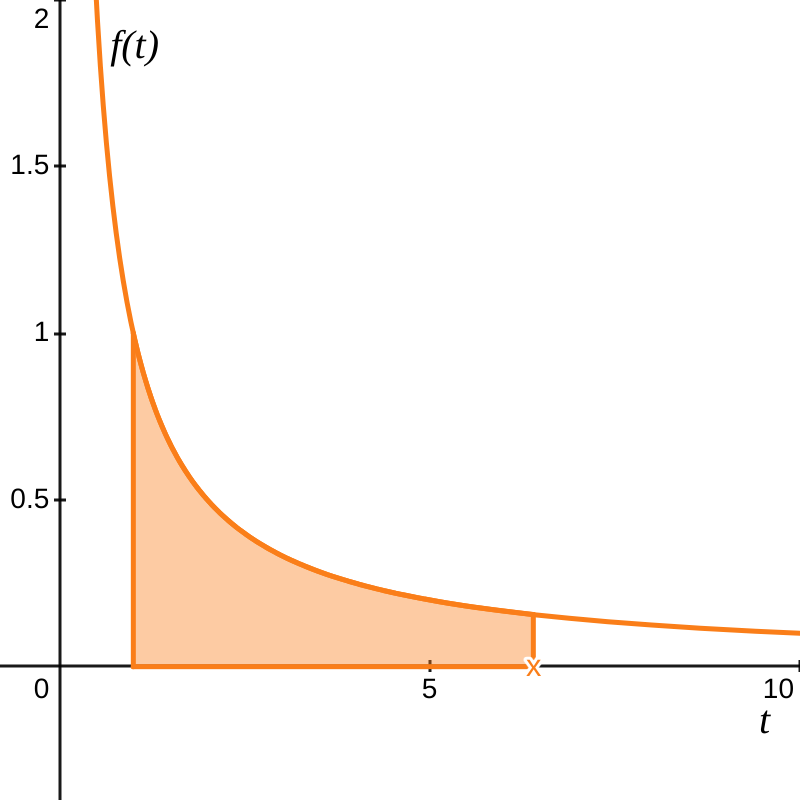
\includegraphics[width=\linewidth]{media/lnx.png}
	\caption{Graphical representation of the integral from $1$ to $x$ of the function $f(t) = \frac{1}{t}$. The variable $x$ can be thought of as a \enquote{slider} which changes how wide the integration window is. An interactive Desmos graph is available at \url{https://www.desmos.com/calculator/drhxhrnnr1}.}
	\label{graph}
\end{figure}

Note that what \enquote{varies} in $A(x)$ is $x$, in other words, that \enquote{slider} which changes how wide our window is. $t$ doesn't vary with $x$, it just defines the function. To clarify this, one might consider taking specific values of $x$. For example, $A(3) = \int_{1}^{3} f(t) dt$ means \enquote{the area encapsulated under the curve drawn by $\frac{1}{t}$ between $t = 1$ and $t = 3$}. This yields a real number with value $1.0986...$.

We \textbf{define} that area function to be the \textit{natural logarithm of $x$} (a name which might as well be meaningless for now), written as $\ln(x) := A(x) = \int_{1}^{x} \frac{1}{t} dt$. Because of the Fundamental Theorem of Calculus, $A'(x) = (\ln(x))' = \frac{1}{x}$ (it can also be proved using the Sandwich theorem). We also define $e$ to be the number that satisfies that $\ln(e) = 1$. 

\newpage

\subsection{Properties of the $\ln(x)$ function.}

Just by looking at the graph it is immediately obvious that for the $\ln(x)$ function to make sense, $x$ must be greater than $0$. We can analyse values between $0$ and $1$ by inverting the integration boundaries and the sign of the result. It's easy to see then that $\ln(x)$ is always an increasing function, and that for values between 0 and 1, its value will be negative. Furthermore, at $x = 1$, its area gets squished into nothingness, so $\ln(1) = 0$.

We can prove the following two properties:

\begin{itemize}
	\item $\ln(ax) = \ln(a) + \ln(x)$ for all $a, x \in \mathbb{R}^+$.
	\item $\ln(x^{\frac{p}{q}}) = \frac{p}{q} \ln(x)$ for all $\frac{p}{q} \in \mathbb{Q}$ and $x \in \mathbb{R}^+$.
\end{itemize}

\subsubsection{Proof of $\ln(ax) = \ln(a) + \ln(x)$.}

We start from taking the derivative of $\ln(ax)$:

$$(\ln(ax))' = \frac{1}{ax} \cdot a = \frac{1}{x} = (\ln(x))'$$

This implies that

$$(\ln(ax) - \ln(x))' = 0$$

meaning

$$\ln(ax) - \ln(x) = c \textrm{ (constant)}$$

To obtain the value of $c$, we can evaluate these functions at $x = 1$.

$$\ln(a) - \ln(1) = c \iff c = \ln(a)$$

That is to say

$$\ln(ax) = \ln(a) + \ln(x)$$

This method also works for proving that $\ln(\frac{x}{a}) = \ln(x) - \ln(a)$. Note that this works for \textit{every positive real number}. 

\subsubsection{Proof of $\ln(x^{\frac{p}{q}}) = \frac{p}{q} \ln(x)$}

Starting again from its derivative,

$$\ln(x^{\frac{p}{q}})' = \frac{1}{x^{\frac{p}{q}}} \frac{p}{q} x^{\frac{p}{q} - 1} = \frac{p}{q} \frac{1}{x} = \frac{p}{q} (\ln(x))'$$

Again, we substract the first and the last derivatives to get zero, meaning that $\ln(x^{\frac{p}{q}}) - \ln(x) = c$ with constant $c$. In this case, the constant turns out to be $c = 0$, leaving

$$\ln(x^{\frac{p}{q}}) = \frac{p}{q} \ln(x)$$

This is valid if $x > 0$ and if $\frac{p}{q} \in \mathbb{Q}$. Still, no real exponents to be found anywhere.

\subsection{The exponential function.}

By these properties, we can confidently say that:

$$\ln(e^2) = 2\ln(e) = 2$$
$$\ln(e^3) = 3\ln(e) = 3$$
$$\ln(e^4) = 4\ln(e) = 4$$
$$\ln(e^{q}) = q, \forall q \in \mathbb{Q}$$

Now we define the \textit{exponential function} to be the inverse of the natural logarithm function: $\exp(x) := \ln^{-1}(x)$. Think of the term \textit{exponential} as a name instead of an adjective. By this definition and by the previous results:

$$\exp(2) = \ln^{-1}(2) = e^2$$
$$\exp(3) = \ln^{-1}(3) = e^3$$
$$\exp(4) = \ln^{-1}(4) = e^4$$

It can be proved that the $\exp(x)$ function shares a lot of similarities with raising $e$ to a power in this regard. The usual properties of exponents transfer into this function.

$$\exp(a + b) = \exp(a\cdot b)$$
$$\exp(a \cdot b) = \exp(a)^b$$
$$\exp\left(\frac{1}{2}\right) = \sqrt{e}$$
$$\exp(-1) = e^{-1}$$

Because of this bizarre correlation, it is almost universal to write $\exp(x)$ as $e^x$. However, $\ln: (0, \infty) \to \mathbb{R}$, and hence $\exp: \mathbb{R} \to (0, \infty)$. In other words, we can evaluate $\exp(x)$ at irrational $x$ values. This isn't a problem for $\exp(x)$, but to say that $e^x$ can have an irrational power implies redefining what \enquote{power} even means.

In essence, we'll define every power with real exponent in terms of $\ln$ and $\exp$. Taking advantage of some notational abuse, we say that:

$$e^x := \exp(x)$$
$$a^x := \exp(x\cdot \ln(a)) = e^{x\cdot \ln(a)}$$

where $a\in \mathbb{R}^+$ and $x\in \mathbb{R}$. Note that $-a^x \in \mathbb{R}$, whereas $(-a)^x \in \mathbb{C}$. This is our first formal definition of $e$:

$$e := \exp(1) = \ln^{-1}(1) \iff \ln(e) = \int_{1}^{e} \frac{1}{t} dt = 1$$

\subsection{Other definitions of $e$.}

As with many things in math, what you define in one occasion turns up in other unexpected places. $e$ was originally discovered in the study of interest rates over different periods of time by Bernoulli.

$$\exp(x) = \lim_{n \to \infty} \left(1 + \frac{x}{n}\right)^n$$

$e$ is characteristic of those phenomena in nature where the rate of change of some variable depends on the value of that variable. Expressed through differential equations, $\exp(x)$ is the solution to:

\begin{equation}
	\begin{cases}
		f'(x) = f(x) \\
		f(0) = 1
	\end{cases}
\end{equation}

If we tried to examine $f$ through its Taylor expansion, we would get another definition for the exponential:

$$\exp(x) = \lim_{n \to \infty} \sum\limits_{k = 0}^{n} \frac{x^k}{k!}$$

\newpage

\section{Complex numbers.}

Complex numbers are also an insanity-inducing topic for those unprepared. The student gets told during their whole life that \enquote{negative numbers don't have square roots} just for one day to throw everything out the window and say they magically do. Not only that, the explanation is rather poor too. The usual definition goes \enquote{let $i = \sqrt{-1}$}, which, when seen from afar, seems like a lazy brutish way of solving the problem. Of course, complex numbers also came to existance through a historical process, but we prefer to offer the already-generalized and well defined set directly.

We define the complex numbers $\mathbb{C}$ as an algebra over the $\mathbb{R}^2$ vector space, with its two operations being:

\begin{itemize}
	\item Addition: $(a, b) + (c, d) = (a + c, b + d)$.
	\item Product: $(a, b) \cdot (c, d) = (ac - bd, ad + bc)$.
\end{itemize}

From now on, the complex number $(a, b)$ will be written as $a + bi$, and we will call $a$ its \textit{real} part and $b$ its \textit{imaginary} part. Note that $i^2 = (0, 1) \cdot (0, 1) = (0 \cdot 0 - 1 \cdot 1, 0 \cdot 1 + 1 \cdot 0) = (-1, 0) = -1$. Because of this fact and, again, through some notational abuse, $i = \sqrt{-1}$.

\subsection{Polar coordinates.}

If instead of having the components of a complex number $z$ we were given its length $|z|$ (also called its \textit{modulus}) and the angle $\alpha$ its vector forms with the real axis (also called its \textit{argument}), we could derive its coordinates using basic trigonometry (see Section \ref{trig}) and get that

$$z = |z| \cdot (\cos(\alpha) + i\cdot \sin(\alpha))$$

We are now ready to prove Euler's formula.

\newpage

\section{La fórmula de Euler.}

Estamos a punto de probar que $\exp(ix) = \cos(x) + i\sin(x)$ de dos maneras distintas.

\subsection{Demostración por ecuaciones diferenciales.}

Primero establecemos que $f$ y $g$ son:

\begin{equation}
\begin{cases}
	f(x) = \cos(x) + i\sin(x) \\
	g(x) = \exp(ix)
\end{cases}
\end{equation}

Podemos ver que cuando evaluamos en $x = 0$, obtenemos el mismo resultado

\begin{equation}
\begin{cases}
	f(0) = \cos(0) + i\sin(0) = 1 \\
	g(0) = \exp(0\cdot i) = 1
\end{cases}
\end{equation}

Por supuesto, demostrarlo para un valor está lejos de demostrarlo para todos los valores, sin embargo, nótese que

\begin{equation}
\begin{cases}
	f'(x) = -\sin(x) + i\cos(x) = i(\cos(x) + i\sin(x)) = if(x) \\
	g'(x) = i\exp(ix) = ig(x)
\end{cases}
\end{equation}

Dos funciones que satisfacen la misma ecuación diferencial para la misma condicion inicial están destinadas a ser iguales, así que

$$\exp(ix) = \cos(x) + i\sin(x)$$

\subsection{Demostración por serie de Taylor.}

Podemos escribir la expansión de Taylor de cada término:

$$\cos(x)  =  \sum\limits_{n=0}^{\infty} \frac{D^n(\cos(x))_{x=0}}{n!} x^n = 1 - \frac{x^2}{2!} + \frac{x^4}{4!} - \frac{x^6}{6!} + \cdots$$
$$i\sin(x) = i\sum\limits_{n=0}^{\infty} \frac{D^n(\sin(x))_{x=0}}{n!} x^n = ix - \frac{ix^3}{3!} + \frac{ix^5}{5!} - \frac{ix^7}{7!} + \cdots$$
$$\exp(ix) =  \sum\limits_{n=0}^{\infty} \frac{(ix)^n}{n!} = 1 + ix - \frac{x^2}{2!} - \frac{ix^3}{3!} + \frac{x^4}{4!} + \frac{ix^5}{5!} - \frac{x^6}{6!} - \frac{ix^7}{7!} + \cdots$$

Es inmediatamente obvio que

$$\exp(ix) = \cos(x) + i\sin(x)$$

\subsection{Notación polar compleja.}

Gracias a esto tenemos una forma muy conveniente y elegante de expresar números complejos. Regresando a las coordenadas polares, cuando un número complejo $z$ era representado por su longitud $|z|$ y su ángulo $\alpha$, teníamos que

$$z = |z| \cdot (\cos(\alpha) + i\sin(\alpha))$$

Con el conocimiento adquirido, está claro que podemos expresar esto como

$$z = |z| \cdot \exp(i\alpha)$$

O, si se prefiere,

$$z = |z| \cdot e^{i\alpha}$$

Et voilá

$$1\cdot e^{i\pi} = \cos(\pi) + i\sin(\pi) = -1 + 0i = -1$$
$$e^{i\pi} = -1$$

\newpage

\section{The underlying meaning.}

Our explanation so far has relied on analythic methods, and, although consistent within itself, one could reasonably argue that it is as obscure as any other one. We now give each concept semantical meaning, such that the reader comes out convinced that what has been seen until now is not only fair, but also somewhat intuitive.

\subsection{Exponential phenomena.}

One of the ways we can categorize different magnitudes is by how they change and develop. The age of a person increases linearly, this means that it doesn't matter whether someone turns 19 or 91, neither whether that happens in 2025 or in 1320; in every case, the rate of change has remained constant: one year per year.

We say a variable grows \textit{exponentially} when its rate of change is proportional to the value of the variable itself. That is, if the variable is equal to 3, then its rate of change will be proportional to 3. This doesn't seem very impressive until you stop to consider its implications and run the numbers. An example of exponential growth (also called \textit{geometric growth} when talking about discrete cases) is the sequence:

$$1, 4, 16, 64, 256, 1024, 4096, 16384...$$

Note that already on the fith term we're on four figures.

We've previously said that real exponents make no sense (at least before introducing the $\exp(x)$ and $\ln(x)$ functions). While this holds true, it is also true that many real world continuous phenomena exhibit an exponential nature. If we stand faithful to our scientific spirit of inquiry, these kind of phenomena should be taken into account before any notion of $\ln(x)$ and $\exp(x)$ is developed. Let us just create a fiction in which, in some way, we got to a formalisation of real exponents that doesn't have anything to do with these two functions, for example, by \enquote{filling in the holes} in the function $f(x) = 4^x$ for $x \in \mathbb{Q}$ such that $x\in \mathbb{R}$ (making it continuous).

We can analyse the derivative of $f(x) = 4^x$ to find its rate of change and get that:

$$f'(x) = 4^x \cdot 1.386294...$$

As expected, its rate of change is proportional to its value, however, the proportionality constant ($1.386294...$) is quite bizarre. It's also worth saying that this proportionality constant varies depending on the base of the exponential. If we had instead used $g(x) = 7^x$, we would've found that

$$g'(x) = 7^x \cdot 1.945910...$$

\newpage

A natural question that comes to mind when pondering about how one would express this constant in terms of the base is to find a base which makes the constant equal to $1$, this means, not only having an exponential function whose rate of change is \textit{proportional} to its current value, but also one that makes it \textit{exactly equal} to its current value. Surprisingly, the value of this base turns out to be $h(x) = e^x$.

$$h'(x) = e^x$$

Knowing this, we can derive the general expression for the derivative of $F(x) = a^x$. First, note that

$$e^{\log_e(a)} = a$$

This has NOTHING to do with the $\ln(x)$ function. Think of $\log_e(a)$ as any other logarithm which just happens to have base $e$. You can formulate it in the usual \enquote{To what power do you have to raise the number $e$ to get $a$?}. We are allowed to write then that

$$F(x) = a^x = [e^{\log_e(a)}]^x = e^{\log_e(a)\cdot x}$$

If we take its derivative and apply the chain rule,

$$F'(x) = e^{\log_e(a)\cdot x} \cdot \log_e(a)$$

(We know $e^x$ to be its own derivative because that's pretty much how we've defined $e$). Substituting back $a^x$, we get that

$$F'(x) = (a^x)' = a^x \cdot \log_e(a)$$

Recovering the knowledge we obtained from previous sections, it is possible to rewrite this as

$$(a^x)' = a^x \cdot \ln(a)$$

But notice that this is somewhat retconning. The function $\log_e(x)$ isn't the same as $\ln(x)$, as the former works on the realm of rational numbers, whereas the latter works with real numbers. Only after having defined what $\ln(x)$ is can we extend $\log_e(x)$ to mean $\ln(x)$.

Rest assured, after having rigorously defined and proved everything, we can write things in whatever order we want, but this must only be done once the student has a solid understanding on why these backwards compatibilities work.

On a less technical note we would like to point out that choosing $e^x$ to represent exponential phenomena in disciplines like physics or statistics is a merely aesthetical choice. One could very much express $2^3$ as $\pi^{\log_{\pi}(2)\cdot 3}$, it's just that when choosing $e^x$, only the non-cluttering constants --- the ones with actual semantic meaning in the universe --- remain.

\newpage

Take exponential decay. If you have a radioactive material, you can measure how many radioactive isotopes it has ($N_0$). With the passage of time ($t$), some of those isotopes will undergo radioactive decay, transforming into other elements or isotopes and leaving a smaller amount of radioactive isotopes in the material ($N(t)$). This process is also an exponential, and thus can be expressed by the following differential equation:

$$N'(t) = -\lambda N(t)$$

One possible solution to this equation is

$$N(t) = N_0 a^{-ct}$$

Where $c = \lambda \cdot \log_a(e)$. This is, by all means, a valid solution. It's only problem, as we've said, is an aesthetic one. What does $c$ mean? Would one know anything about the phenomenon being described just by glancing at this constant? Absolutely not. If we instead express it this way

$$N(t) = N_0 e^{-\lambda t}$$

Suddenly there are no \enquote{clutter constants} and, more importantly, $\lambda$ takes semantic meaning. In the case of radioactive decay, $\lambda$ is called the \textit{disintegration constant} or \textit{rate constant}. This is not only meaningful for $\lambda$ itself, but for all the magnitudes derived from $\lambda$. For example, $t_{1/2} = \frac{\ln(2)}{\lambda}$ is called the \textit{half life} of the quantity, and it describes the amount of time necessary for the amount $N$ to be cut in half. Could have we expressed the same thing by carrying a factor of $log_a(e)$ the whole time? Absolutely, but then our definition of half life would be something like \enquote{the amount of time necessary for the amount $N$ to be cut in half divided by $\log_a(e)$}. This definition just feels wrong and muddled, whereas the other one seems to carry some objective meaning, as if the constant $e$ was just the \textit{natural} option for deciding a base. This is what makes the natural logarithm \textit{natural}.

To summarize, exponential variables are those whose rate of change is proportional to the variable's value itself, and $e$ is the number which satisfies that that proportionality constant is $1$, which makes it the \textit{natural} way of expressing many equations in physics.

\subsection{Complex numbers as rotations.}

When first introduced to complex numbers, one of the first strange decisions that stand out about their definition is their position on the complex plane. Although any ordered pair can be plotted in a graph, it doesn't seem obvious why $i$ should be one step up from $0$ perpendicular to the real axis. However, when we shift our perspective on numbers to thinking of them as \textit{actions}, this not only becomes a reasonable outcome, but the only possible one.

If one is familiar with simple $\mathbb{R}^2$ vectors, one will already see how numbers can be seen this way. Multiplying a vector by a positive number is \textit{scaling} it, making it bigger or smaller while preserving the way it \enquote{points} to. Similarly, multiplying it by a negative number is doing the same thing but also \enquote{flipping} its direction, or rotating it by $180^{\circ}$.

But what is a $180^{\circ}$ rotation if not two consecutive $90^{\circ}$ rotations? If multiplying by $-1$ yields a $180^{\circ}$ rotation, whatever number represents a $90^{\circ}$ rotation must be, in a sense, the square root of $-1$. This notion of multiplication (of numbers) turning into addition (of angles) should already give away a hint that exponentials will sooner or later be useful as a model.

If one isn't convinced by this argument, note the following. If $z = a + bi$, then $i\cdot z = -b + ai$. This coordinate transformation is exactly the same as a $90^{\circ}$ counter-clockwise rotation ($(x, y) \to (-y, x)$). This concept can be expanded further onto other complex numbers, however our case only requires for us to understand the action of $i$.

\subsection{Complex exponentials.}

This is perhaps the hardest part of all to visualize, so we shall use a physics analogy. It can be useful to interpret $f(t) = \exp(it)$ as the position of a particle in the complex plane at a given point in time, and its derivative $f'(t) = i\exp(it)$ as its velocity. It is worth noting that, at every position, the particle's velocity vector forms a $90^{\circ}$ angle with its position vector (because $f'(t) = i\cdot f(t)$, that is, a $90^{\circ}$ counter-clockwise rotation). One can visualize the particle \enquote{orbiting} the origin in a circular motion (Figure \ref{rot}).

\begin{figure}[H]
	\centering
	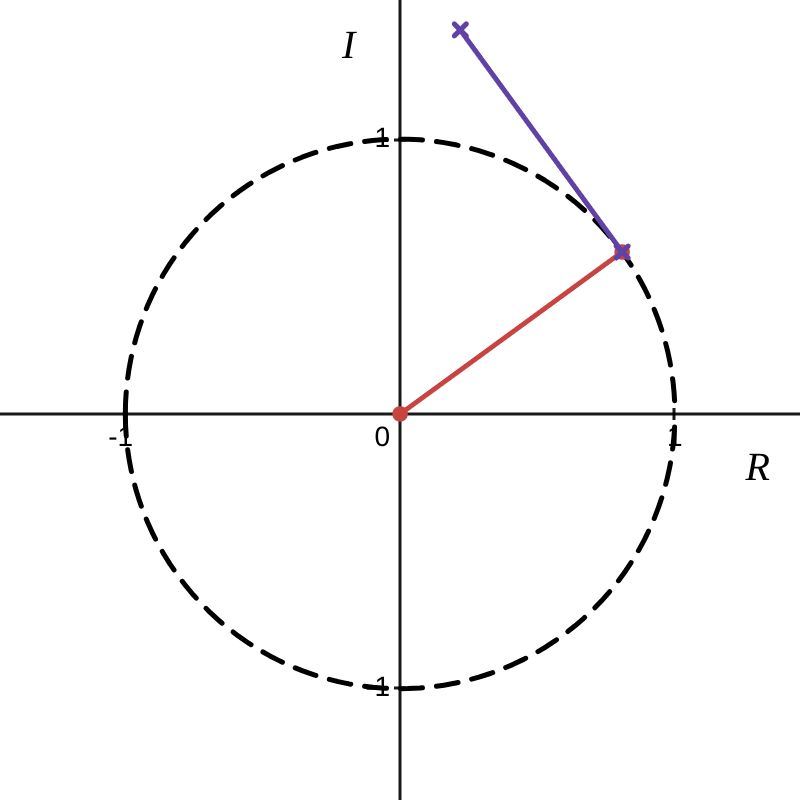
\includegraphics[width=\linewidth]{media/rotation.png}
	\caption{Particle on the complex plane with position $\exp(it)$ (shown in red) and velocity $i\exp(it)$ (shown in purple). In the beginning, $f(0) = 1$. After an infinitesimal nudge in time, the particle will move perpendicular to its position vector (along its velocity vector). As we know from physics, this is the setup for circular motion. An interactive Desmos graph is available at \url{https://www.desmos.com/calculator/8npnlxgjba}.}
	\label{rot}
\end{figure}

What Euler's formula tells us is that the angle the particle's position vector has swept at time $t$ is \textit{exactly} $t$. So, after 2 seconds, the particle forms a 2 radian angle with the real axis; after $\pi$ seconds, the particle forms a $\pi$ radian angle with the real axis (which coincides with the point $-1 + 0i$), etc.

Once again, the exponential function here is not a fundamental choice. We could've chosen the golden ratio $\phi$ as a base, making $f(t) = \phi^{it}$ and $f'(t) = \ln(\phi) \cdot \phi^{it}$. The only difference is that in this case the swept angles don't match the elapsed time. Using this function, we get to EulErik's formula (named like that for no particular reason):

$$\phi^{i\frac{\pi}{\log_{\phi}(e)}} = -1$$

\section{Conclusion.}

To compress everything seen thus far into a simple summary:

\begin{itemize}
	\item Complex numbers provide a way to express rotations in the complex plane. Specifically, $i$ means a $90^{\circ}$ counter-clockwise rotation.
	\item The exponential function ($\exp(x)$ or $e^x$) provides a way to express phenomena whose rate of change is the same as their current value. Its most fundamental characteristic is the fact that its derivative is equal to itself.
	\item $e^{it}$ is the point that results from rotating a point around an origin for $t$ time, and because of the already mentioned properties of $\exp(x)$, this particular case satisfies that the elapsed time is the same as the angle swept by the position vector of the point. Another way to express this vector's position is $\cos(x) + i\sin(x)$ (Euler's formula).
	\item $e^{i\pi}$ is the particular case where the point lands on $-1$ (Euler's identity).
\end{itemize}


\end{document}
